\chapter{Case Study} \label{ch:casestudy}

In the supply chain model as mentioned in the methodology section, we are considering the supply chain consisting of 5 Suppliers, 7 Manufacturers, 10 Distributors, and 20 Retailers as our case study. This supply chain model is then subjected to different sources of disruption. The results of the resilience value for modeling with and without the resiliency and robustness enhancers are compared for quantifying the methodology. This case study can be considered for generic design purposes as well. The values of the parameters for the Suppliers are as shown in the Table \ref{tab:Supplier}. The parameters for the manufacturer agent and their corresponding values are shown in the Table \ref{tab:Manufacturer}. The parameters for the distributor agent and the values associated with them are as shown in the Table \ref{tab:Distributor}. The values corresponding to this parameter for the retailer agent is as shown in the Table \ref{tab:Retailer}. The costs such as inventory holding cost and backlog cost together make the total cost (lost) in the supply chain. Theses costs are used for the quantification of our methodology.


\begin{table}[H]
\caption{Parameters of the Supplier}
\label{tab:Supplier}
\begin{center}
\begin{tabular}[b]{|c|c|c|}
	\hline
	Supplier & Raw Material Handling Cost & Response Time \\ \hline
	S1 & 0.45 & High\\ \hline
	S2 & 0.52 & Medium \\ \hline
	S3 & 0.44 & High \\ \hline
	S4 & 0.58 & Low \\ \hline
	S5 & 0.56 & Medium \\ \hline
\end{tabular}
\end{center}
\end{table}

\begin{table}[H]
\caption{Parameters of the Manufacturer}
\label{tab:Manufacturer}
\begin{center}
\begin{tabular}[b]{|c|c|c|}
	\hline
	Manufacturer & Inventory Holding Cost & Response Time \\ \hline
	M1 & 0.51 & Low\\ \hline
	M2 & 0.41 & Medium \\ \hline
	M3 & 0.43 & Medium \\ \hline
	M4 & 0.57 & High \\ \hline
	M5 & 0.49 & Low \\ \hline
	M6 & 0.55 & High \\ \hline
	M7 & 0.48 & Low \\ \hline
\end{tabular}
\end{center}
\end{table}

\begin{table}[H]
\caption{Parameters of the Distributor}
\label{tab:Distributor}
\begin{center}
\begin{tabular}[b]{|c|c|c|c|}
	\hline
	Distributor & Inventory Holding Cost & Order Fulfillment Rate & Response Time \\ \hline
	D1 & 0.46 & High & Medium\\ \hline
	D2 & 0.51 & High & High \\ \hline
	D3 & 0.44 & Low & Low \\ \hline
	D4 & 0.52 & High & High \\ \hline
	D5 & 0.48 & Low & Medium \\ \hline
	D6 & 0.49 & Low & Low \\ \hline
	D7 & 0.57 & High & Low \\ \hline
    D8 & 0.41 & High & Medium \\ \hline
    D9 & 0.48 & High & High \\ \hline
    D10 & 0.53 & Low & Low \\ \hline
\end{tabular}
\end{center}
\end{table}

\begin{table}[H]
\caption{Parameters of the Retailer}
\label{tab:Retailer}
\begin{center}
\begin{tabular}[b]{|c|c|}
	\hline
	Retailer & Response Time \\ \hline
	R1 & Low \\ \hline
	R2 & Medium \\ \hline
	R3 & Low \\ \hline
	R4 & High \\ \hline
	R5 & High \\ \hline
	R6 & Medium \\ \hline
	R7 & High \\ \hline
	R8 & Low \\ \hline
	R9 & Low \\ \hline
	R10 & Medium \\ \hline
	R11 & High \\ \hline
	R12 & Low \\ \hline
	R13 & Medium \\ \hline
	R14 & Medium \\ \hline
	R15 & High \\ \hline
	R16 & High \\ \hline
	R17 & High \\ \hline
	R18 & Low \\ \hline
	R19 & High \\ \hline
	R20 & Medium \\ \hline
\end{tabular}
\end{center}
\end{table}

\newpage
\section{The Base Model Connections}
The four agent types are connected to each other to form 5 supply chains in the different regions throughout the country for a company. In the base model, the connections of the agents is as shown in the Fig \ref{Base}. It can be observed from the Fig \ref{Base} that the distributor D1 is shared by three retailers R3, R5 and R15. If there is a disruption in the area of Oregon and the distributor D1 is down due to it, then the retailers R3, R5, and R15 have to select a different distributor facility. They will choose the distributors from D2 to D10 based on who has the best parameter values. Similarly, the distributor agents and manufacturer agents connect to the best available manufacturer agent and supplier agent respectively based on the parameters. In the meantime, the restoration of the disrupted facility is taking place using appropriate mitigation strategies. This is the basic working logic of the whole simulation model. The run time of the simulation for our model is 365 days and the three different scenarios are at distributor level, at manufacturer level, and at supplier level. Theses three scenarios are considered under normal working conditions, under disruption conditions, and under disruption conditions with contingency planning. Out of these three scenarios, we have considered the scenario for disruptions at the manufacturer level.

\begin{figure}[H]
  \centering
  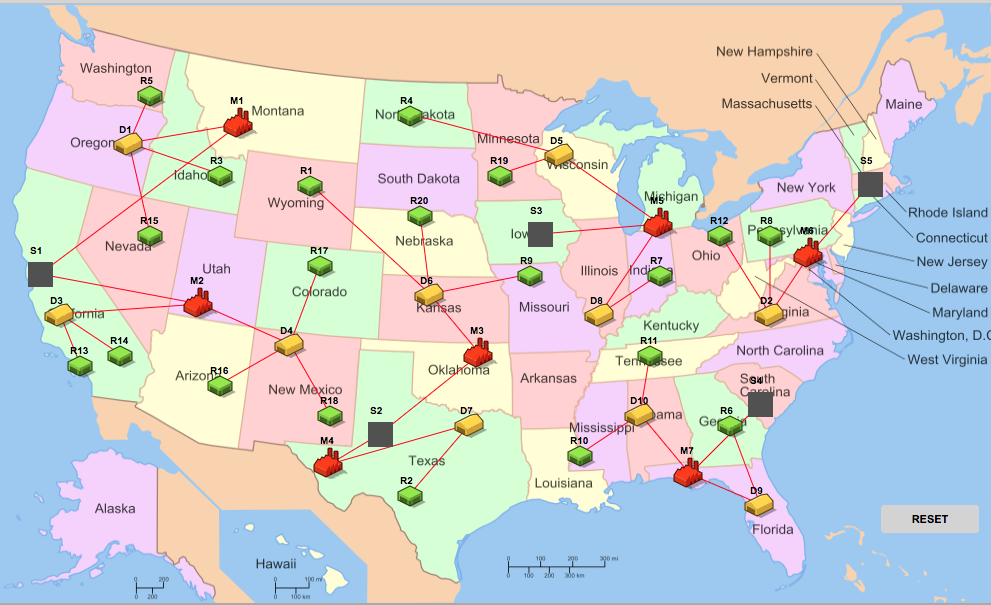
\includegraphics[width=4.0in]{figures/pdf/Basic-connections.png}\\
  \caption{Base Model Agent Connections.}\label{Base}
\end{figure}


\section{Modeling for disruptions at the Manufacturer Level}
 In this model, the connections of the supply chain are as shown in the Fig \ref{Base}. There are three scenarios that can be observed for the behavior of supply chain at the manufacturer level. These scenarios are the supply chain under normal conditions, the supply chain under disruption condition, and the supply chain under disruption condition with contingency planning. The various sources of disruption are considered for these three scenarios. The total costs (lost) and the resiliency values corresponding to these scenarios are calculated.  
 
 \subsection{Supply Chain Performance under Normal Conditions}
In this scenario, the supply chain at manufacturer level is functioning under normal conditions. There exists losses in terms of cost due to the uncertainty of demands and unavailability of the inventory at certain facilities. These losses are due to the inventory holding costs and the backlog costs. The total costs incurred at the three different zones as shown in fig \ref{Base} are \$39,973.4, \$63,139.25, and \$15,842.02 for zones 1, 2, and 3 respectively. The next step is to find out these values under the conditions of disruption. The manufacturing facilities in the three different zones are disrupted at random and the performance of the supply chain is monitored.

 \subsection{Supply Chain Performance under Disruption Conditions}

In this scenario, we have disrupted the different manufacturers which are located in the entire supply chain across the entire geographical United States of America. As these manufacturers are down, the effects of disruption spread throughout the supply chain through the facilities linked with them. This occurs due to the phenomenon known as ripple effect. As the manufacturers supply for the distributors, the distributors are unable to collect the finished goods and fulfill the demand for the retailers associated with them. As a result, the retailers are unable to fulfill the demands of the customers in their region. Thus, a backlog takes place both at the retailers and distributors. The suppliers linked to the manufacturers have to hold the excess raw materials at their facility due to the uncertain duration of recovery of the disrupted facility. The connections before and after the disruption at one such manufacturer facility M2 are shown in the Fig \ref{fig:MLDb} and Fig \ref{fig:MLDa}. The disruption causes the facilities R13, R14, R16, R17, R18, D3, and D4 to become inactive. The supplier S1 gets disconnected from the manufacturer M2.

The lost time and recovery time occurred during different scenarios has a different value. Apart from the loss of time, there are other ramifications such as the backlog cost, inventory holding cost and the loss of customer loyalty. The disruptions take place at the manufacturer level over the period of 365 days. In this period, there are 18 different disruptions which are caused due to the different sources of disruption which are mentioned in the methodology section. This causes a delay of 126 days in the supply chain. Out of these 126 days, the repair time ($T_{\text{N}}$) comprises of 54 days. The lost time ($T_{\text{L}}$) in this scenario is of 72 days. Thus, the recovery time of this scenario is calculated as follows.

\begin{equation}
    T_R = T_N + T_L = 54 + 72 = 126  \label{3.3}
\end{equation}

The total cycle time ($T_{\text{C}}$) in this scenario is of 239 days. The total time of the system now becomes the sum of the total cycle time ($T_{\text{C}}$) and the recovery time ($T_{\text{R}}$). Thus, the resilience value for this scenario is calculated as follows.

\begin{equation}
  R_S = \frac{T}{T_R} = \frac{365}{126} = 2.89  \label{existing}
\end{equation}

The resilience value from the equation \ref{existing} is the existing resilience value ($R_{\text{existing}}$) of the supply chain. The total costs suffered due to the disruptions which comprise of the inventory holding cost and the backlog costs for zones 1, 2, and 3 are \$159,090.8, \$145,987.25, and \$184,948.28 respectively. These heavy losses are suffered due to the absence of mitigation and resilient strategies in the design of the supply chain.

 \begin{figure}[H]
   \centering
    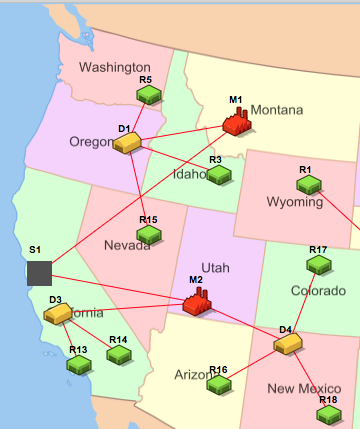
\includegraphics[width=3.0in]{figures/pdf/BeforeM.png} 
    \caption{Manufacturer Level Disruption (Before).}
    \label{fig:MLDb}
\end{figure}

\begin{figure}[H]
    \centering
   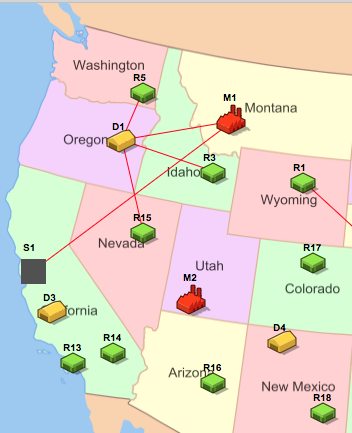
\includegraphics[width=3.0in]{figures/pdf/AfterM.png}
   \caption{Manufacturer Level Disruption (After).}
   \label{fig:MLDa}
\end{figure}

\subsection{Supply Chain Performance under Disruption Conditions with Contingency Planning and Key Indicators Identification}
In this scenario, we have implemented the key indicator identification and contingency planning components into our supply chain. Whenever a disruption takes place, the source of the disruption is identified and a team of management personnel look into the capabilities that need to be strengthened in order to reduce the recovery time. In the meantime, an alternate facility having the least distance, lowest costs, high fulfillment rate, and low response time is selected from the other available facilities. There is transportation cost that is incurred due to alternate facility location. But, this cost is just a small price to pay in order to avoid huge losses if we wait for the damaged facility to be repaired. The lost time is reduced by a drastic amount and thus the total delay caused by the disruption is reduced while keeping the supply chain working simultaneously. Thus, a resilient and robust supply chain is achieved.

In this period, there are 18 different disruptions which are caused due to the different sources of disruption which are mentioned in the methodology section. In this scenario due to the inclusion of resilience techniques such as contingency planning and key indicators identification, there is a delay of 72 days in the supply chain. Out of these 72 days, the repair time ($T_{\text{N}}$) comprises of 54 days. The lost time ($T_{\text{L}}$) in this scenario is of 18 days. Thus, the recovery time of this scenario is calculated as follows.

\begin{equation}
    T_R = T_N + T_L = 54 + 18 = 72  \label{3.3}
\end{equation}

 The total time of the system now becomes the sum of the total cycle time ($T_{\text{C}}$) and the recovery time ($T_{\text{R}}$) which is 365 days. Thus, the resilience value for this scenario is calculated as follows.

\begin{equation}
  R_S = \frac{T}{T_R} = \frac{365}{72} = 5.0694  \label{new}
\end{equation}

The resilience value from the equation \ref{new} is the existing resilience value ($R_{\text{new}}$) of the supply chain. The percentage change in the resilience value can now be calculated as follows.

\begin{equation}
      \% change in resilience = \frac{5.0694 - 2.89}{2.89} * 100 = 75.411 \%  \label{res}
\end{equation}

The equation \ref{res} represents the improvement achieved in the resilience value after incorporating the resilience factors in the supply chain. The total costs suffered due to the disruptions which comprise of the inventory holding cost and the backlog costs for zones 1, 2, and 3 are \$63,606.4, \$82,938.00, and \$43,773.04 respectively. 

Due to the contingency planning, whenever a manufacturing facility is down due to disruption, an alternate manufacturing facility is provided without much loss in time. This enables for the demand of the distributor facilities associated with the disrupted facility to be satisfied so that the demand of the retailers associated with the distributors can be satisfied. If there is a disruption at the manufacturers in the zone 1, then the distribution facilities D1, D3, and D4 get affected as well. Thus, affecting the retailers R3, R5, R13, R14, R15, R16, R17 and R18. Through contingency planning, in times of disruption, the distribution facilities are allocated the manufacturing facility M4 for the fulfillment of their demands such that the supply chain does not come to a halt. The effect of disruption on the manufacturing facilities in the zone 1 is shown in the fig \ref{Z1BD}. The pictorial representation of the contingency planning for zone 1 is shown in the fig \ref{Z1AD}. Similarly, the effects of disruption on the manufacturing facilities of zone 2 and zone 3 can be seen in the figures \ref{Z2BD} and \ref{Z3BD}. The contingency planning for zone 2 and 3 are shown in figures \ref{Z2AD} and \ref{Z3AD}. Through the key indicators identification, the capabilities associated with the source of the disruption can be utilized for mitigating the effects of the disruption. The capabilities are highlighted in the simulation depending on the duration of the disruptions which identifies the source of disruption. This identification of the capabilities in the simulation software is as shown in figure \ref{V1}, \ref{V2}, \ref{V3}, \ref{V4}, and \ref{V5} for the disruption sources (vulnerabilities) as Turbulence, Supplier/Customer disruptions, Resource Limits, Connectivity, and Deliberate threats. This aids in reducing the recovery time of the supply chain from disruption and reducing the losses incurred.

\begin{figure}[H]
  \centering
  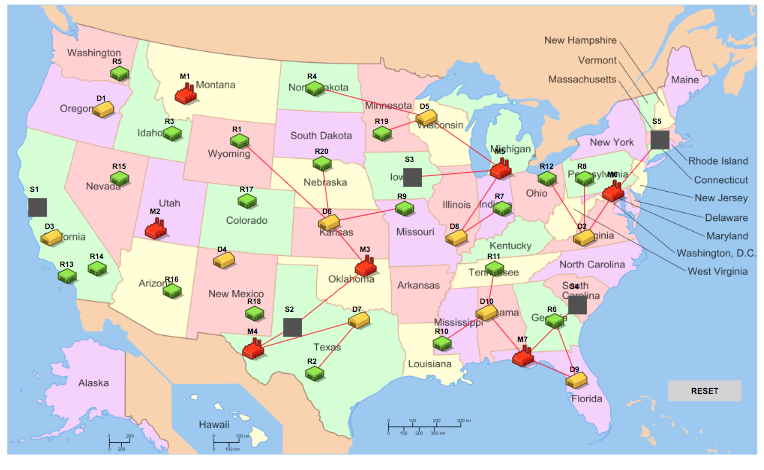
\includegraphics[width=6.5in]{figures/pdf/Z1BD.png}\\
  \caption{Zone 1 during disruption}\label{Z1BD}
\end{figure}  

\begin{figure}[H]
  \centering
  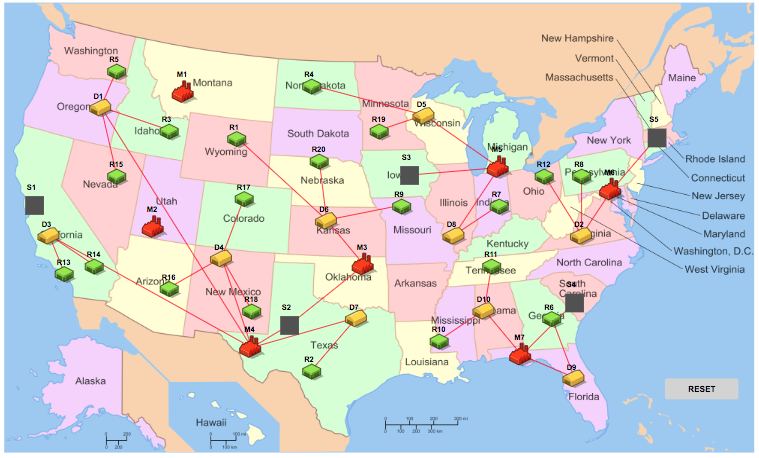
\includegraphics[width=6.5in]{figures/pdf/Z1AD.png}\\
  \caption{Zone 1 after disruption with contingency planning}\label{Z1AD}
\end{figure}  

\begin{figure}[H]
  \centering
  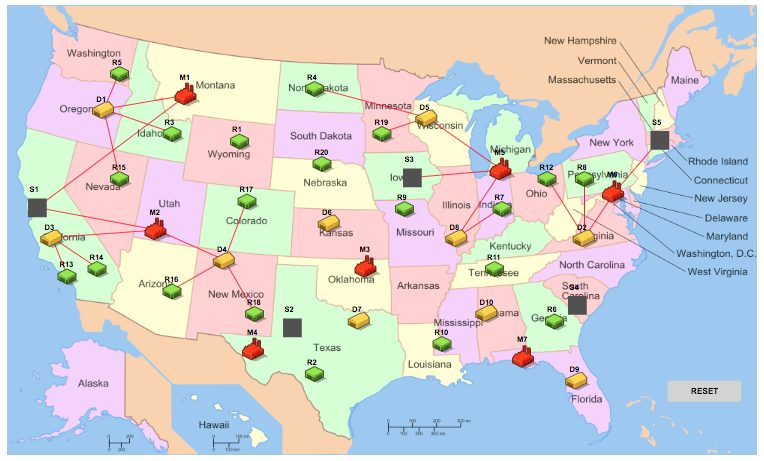
\includegraphics[width=6.5in]{figures/pdf/Z2BD.png}\\
  \caption{Zone 2 during disruption}\label{Z2BD}
\end{figure}  

\begin{figure}[H]
  \centering
  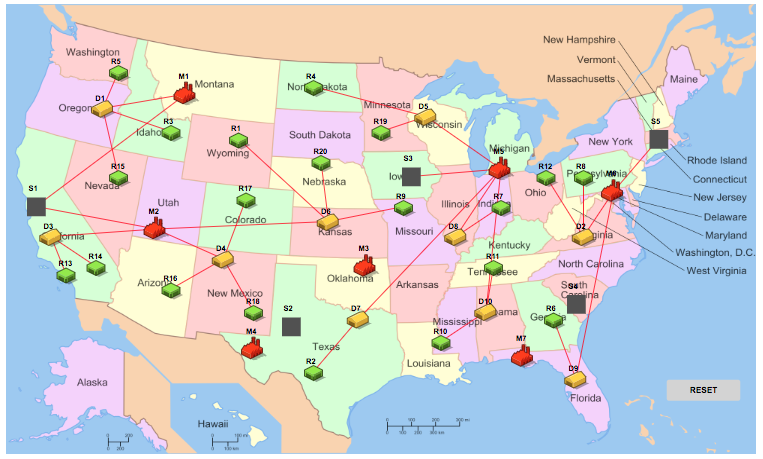
\includegraphics[width=6.5in]{figures/pdf/Z2AD.png}\\
  \caption{Zone 2 after disruption with contingency planning}\label{Z2AD}
\end{figure}  

\begin{figure}[H]
  \centering
  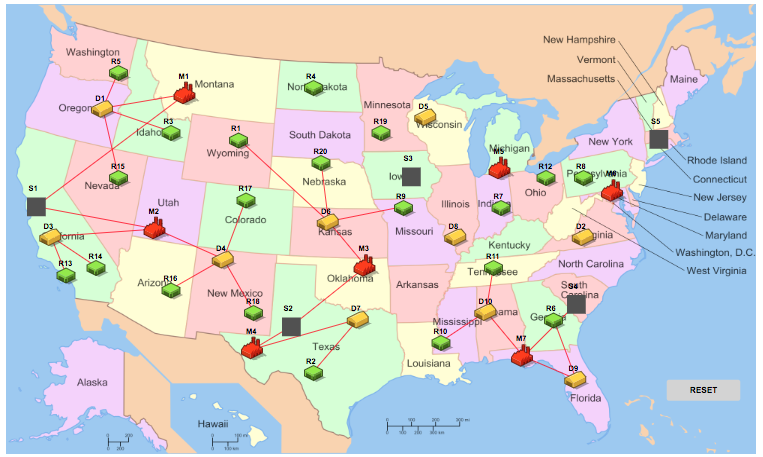
\includegraphics[width=6.5in]{figures/pdf/Z3BD.png}\\
  \caption{Zone 3 during disruption}\label{Z3BD}
\end{figure}  

\begin{figure}[H]
  \centering
  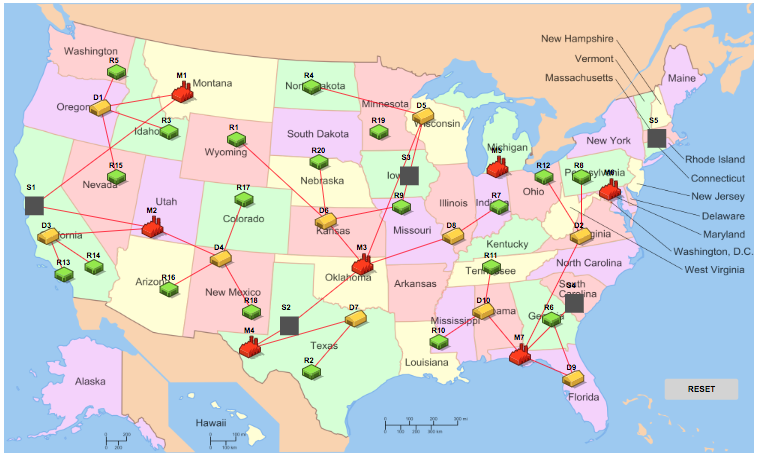
\includegraphics[width=6.5in]{figures/pdf/Z3AD.png}\\
  \caption{Zone 3 after disruption with contingency planning}\label{Z3AD}
\end{figure}  

\begin{figure}[H]
  \centering
  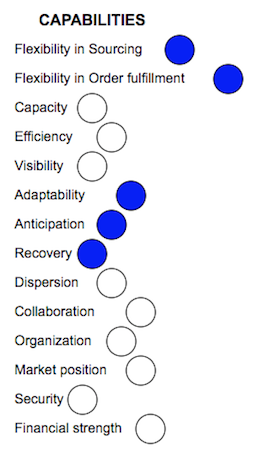
\includegraphics[width=4.5in]{figures/V1.png}\\
  \caption{Capabilities for Vulnerabilities due to Turbulence}\label{V1}
\end{figure}  

\begin{figure}[H]
  \centering
  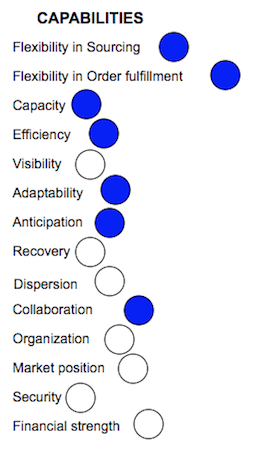
\includegraphics[width=4.5in]{figures/V2.png}\\
  \caption{Capabilities for Vulnerabilities due to Supplier/Customer disruptions}\label{V2}
\end{figure}  

\begin{figure}[H]
  \centering
  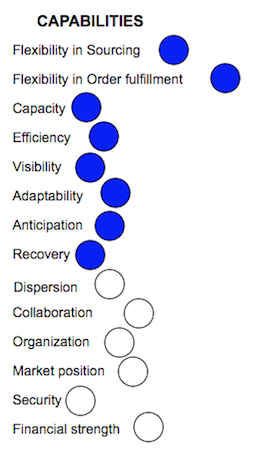
\includegraphics[width=4.5in]{figures/V3.png}\\
  \caption{Capabilities for Vulnerabilities due to Resource Limits}\label{V3}
\end{figure}  

\begin{figure}[H]
  \centering
  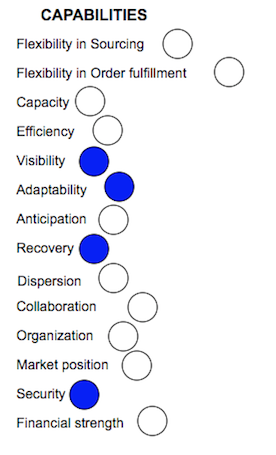
\includegraphics[width=4.5in]{figures/V4.png}\\
  \caption{Capabilities for Vulnerabilities due to Connectivity}\label{V4}
\end{figure}  

\begin{figure}[H]
  \centering
  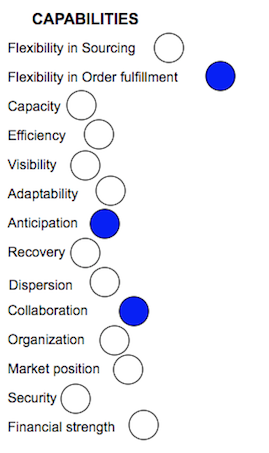
\includegraphics[width=4.5in]{figures/V5.png}\\
  \caption{Capabilities for Vulnerabilities due to Deliberate Threats}\label{V5}
\end{figure}  

\newpage
Among the two, the manufacturer level under disruption with contingency planning and key indicators identification scenario seems to have a better resilience value and less loss in terms of money due to the short recovery time and alternate sourcing. These values are calculated so that the importance of implementing resilience and robustness in the supply chain can be quantified. There can be a huge variation in these values depending on the source of disruption. Thus the resilience values for the disruptions at other levels of the supply chain can be found out as well. It is clearly evident that there is an improvement in the resilience after the inclusion on resilience and robustness components in the design of the supply chain. The total costs incurred at all three scenarios for all three zones of the supply chain model are compared for exhibiting the significance of incorporating the resilience components of contingency planning and key indicators identification. In addition to this, another key observation that can be made through this study is the relationship between the resilience value and the total costs. This relation can be observed in the graph in the fig \ref{G2}. It can be inferred from this graph that higher the resilience value, lesser are the total costs suffered.




\begin{figure}[H]
  \centering
  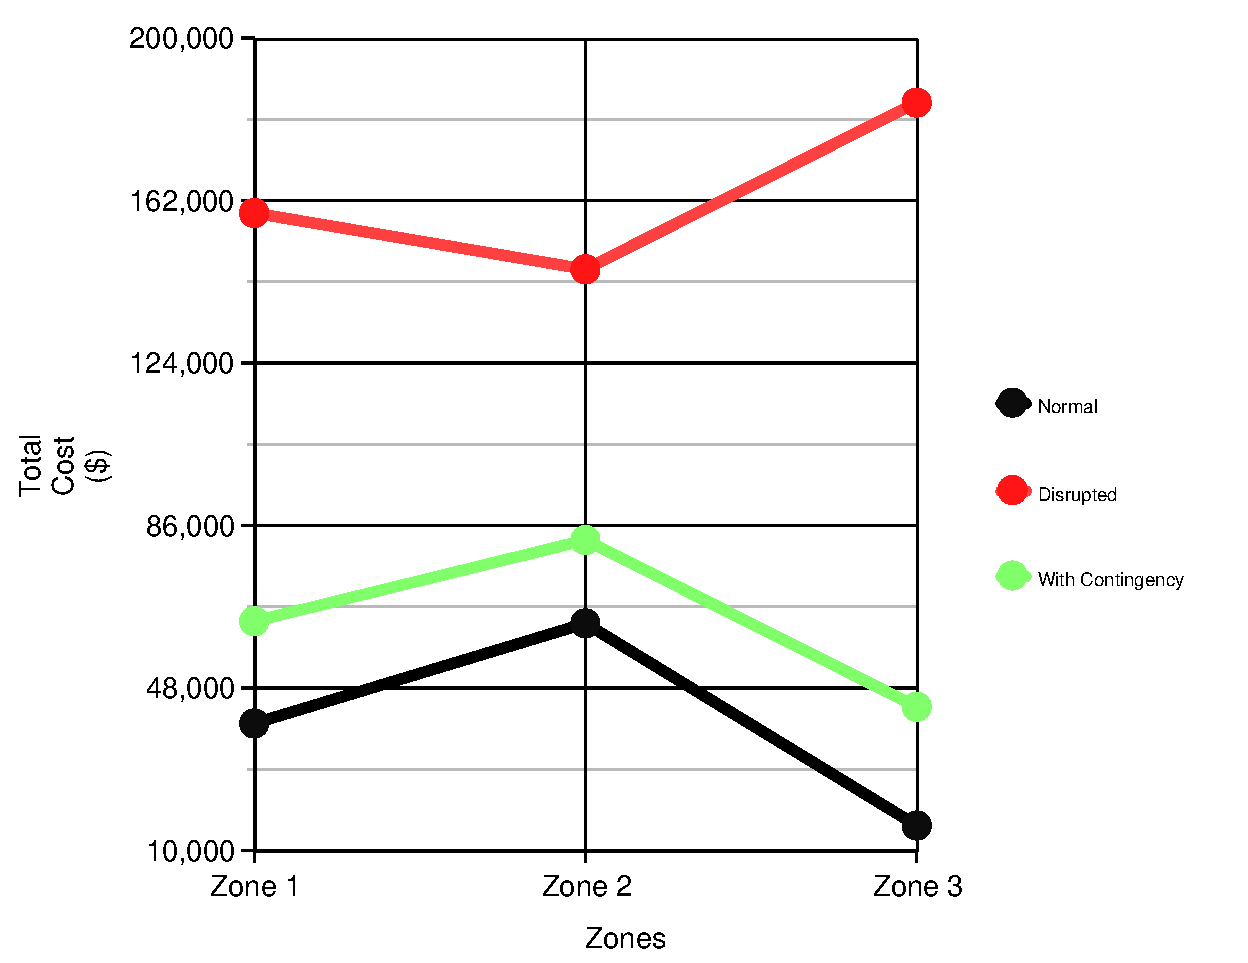
\includegraphics[width=6.5in]{figures/pdf/TotalCosts.pdf}
  \caption{Graph for the total costs for all the three scenarios at the different zones of the Supply Chain Model}\label{G1}
\end{figure}  

\begin{figure}[H]
  \centering
  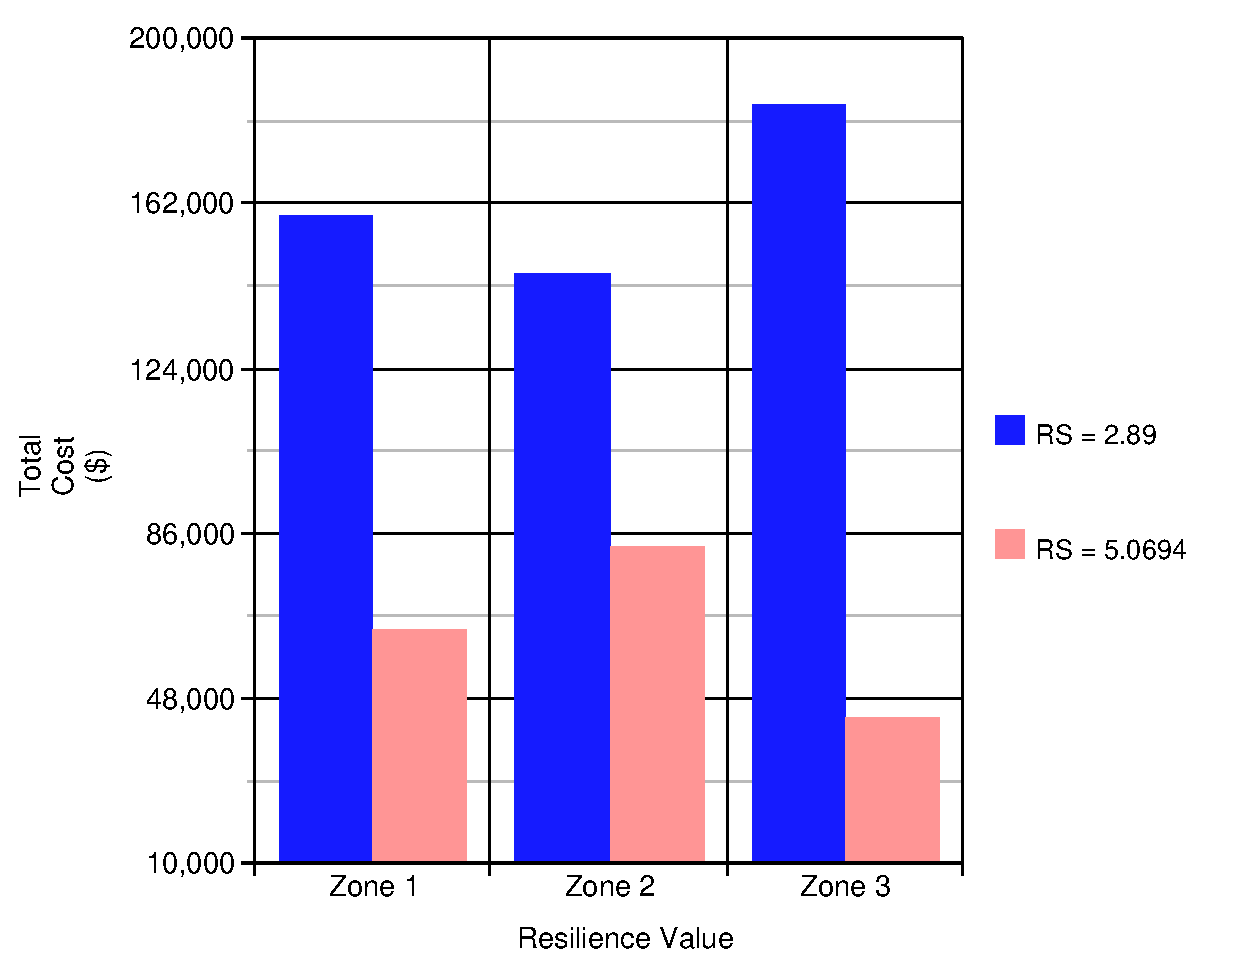
\includegraphics[width=6.5in]{figures/pdf/RVC.pdf}
  \caption{Resilience value VS Total Costs for different zones of the Supply Chain Model}\label{G2}
\end{figure}  


